Surrounded by a superconducting solenoid producing a 2 Tesla magnetic field, the Inner Detector measures the trajectories of charged particles and is composed of three layers of tracking detectors.
%Closest to the beam line the silicon Pixel detector is used for fine grain track hit discrimination.
%A larger grain silicon strip detector, the Semiconductor Tracker, then sits in the next most outer layer.
%And finally in the outer most layer a large volume drift tube detector, the Transition Radiation Tracker, provides tracking and particle discrimination.  
\begin{figure}[h]
  \begin{center}
    \makebox[\textwidth][c]{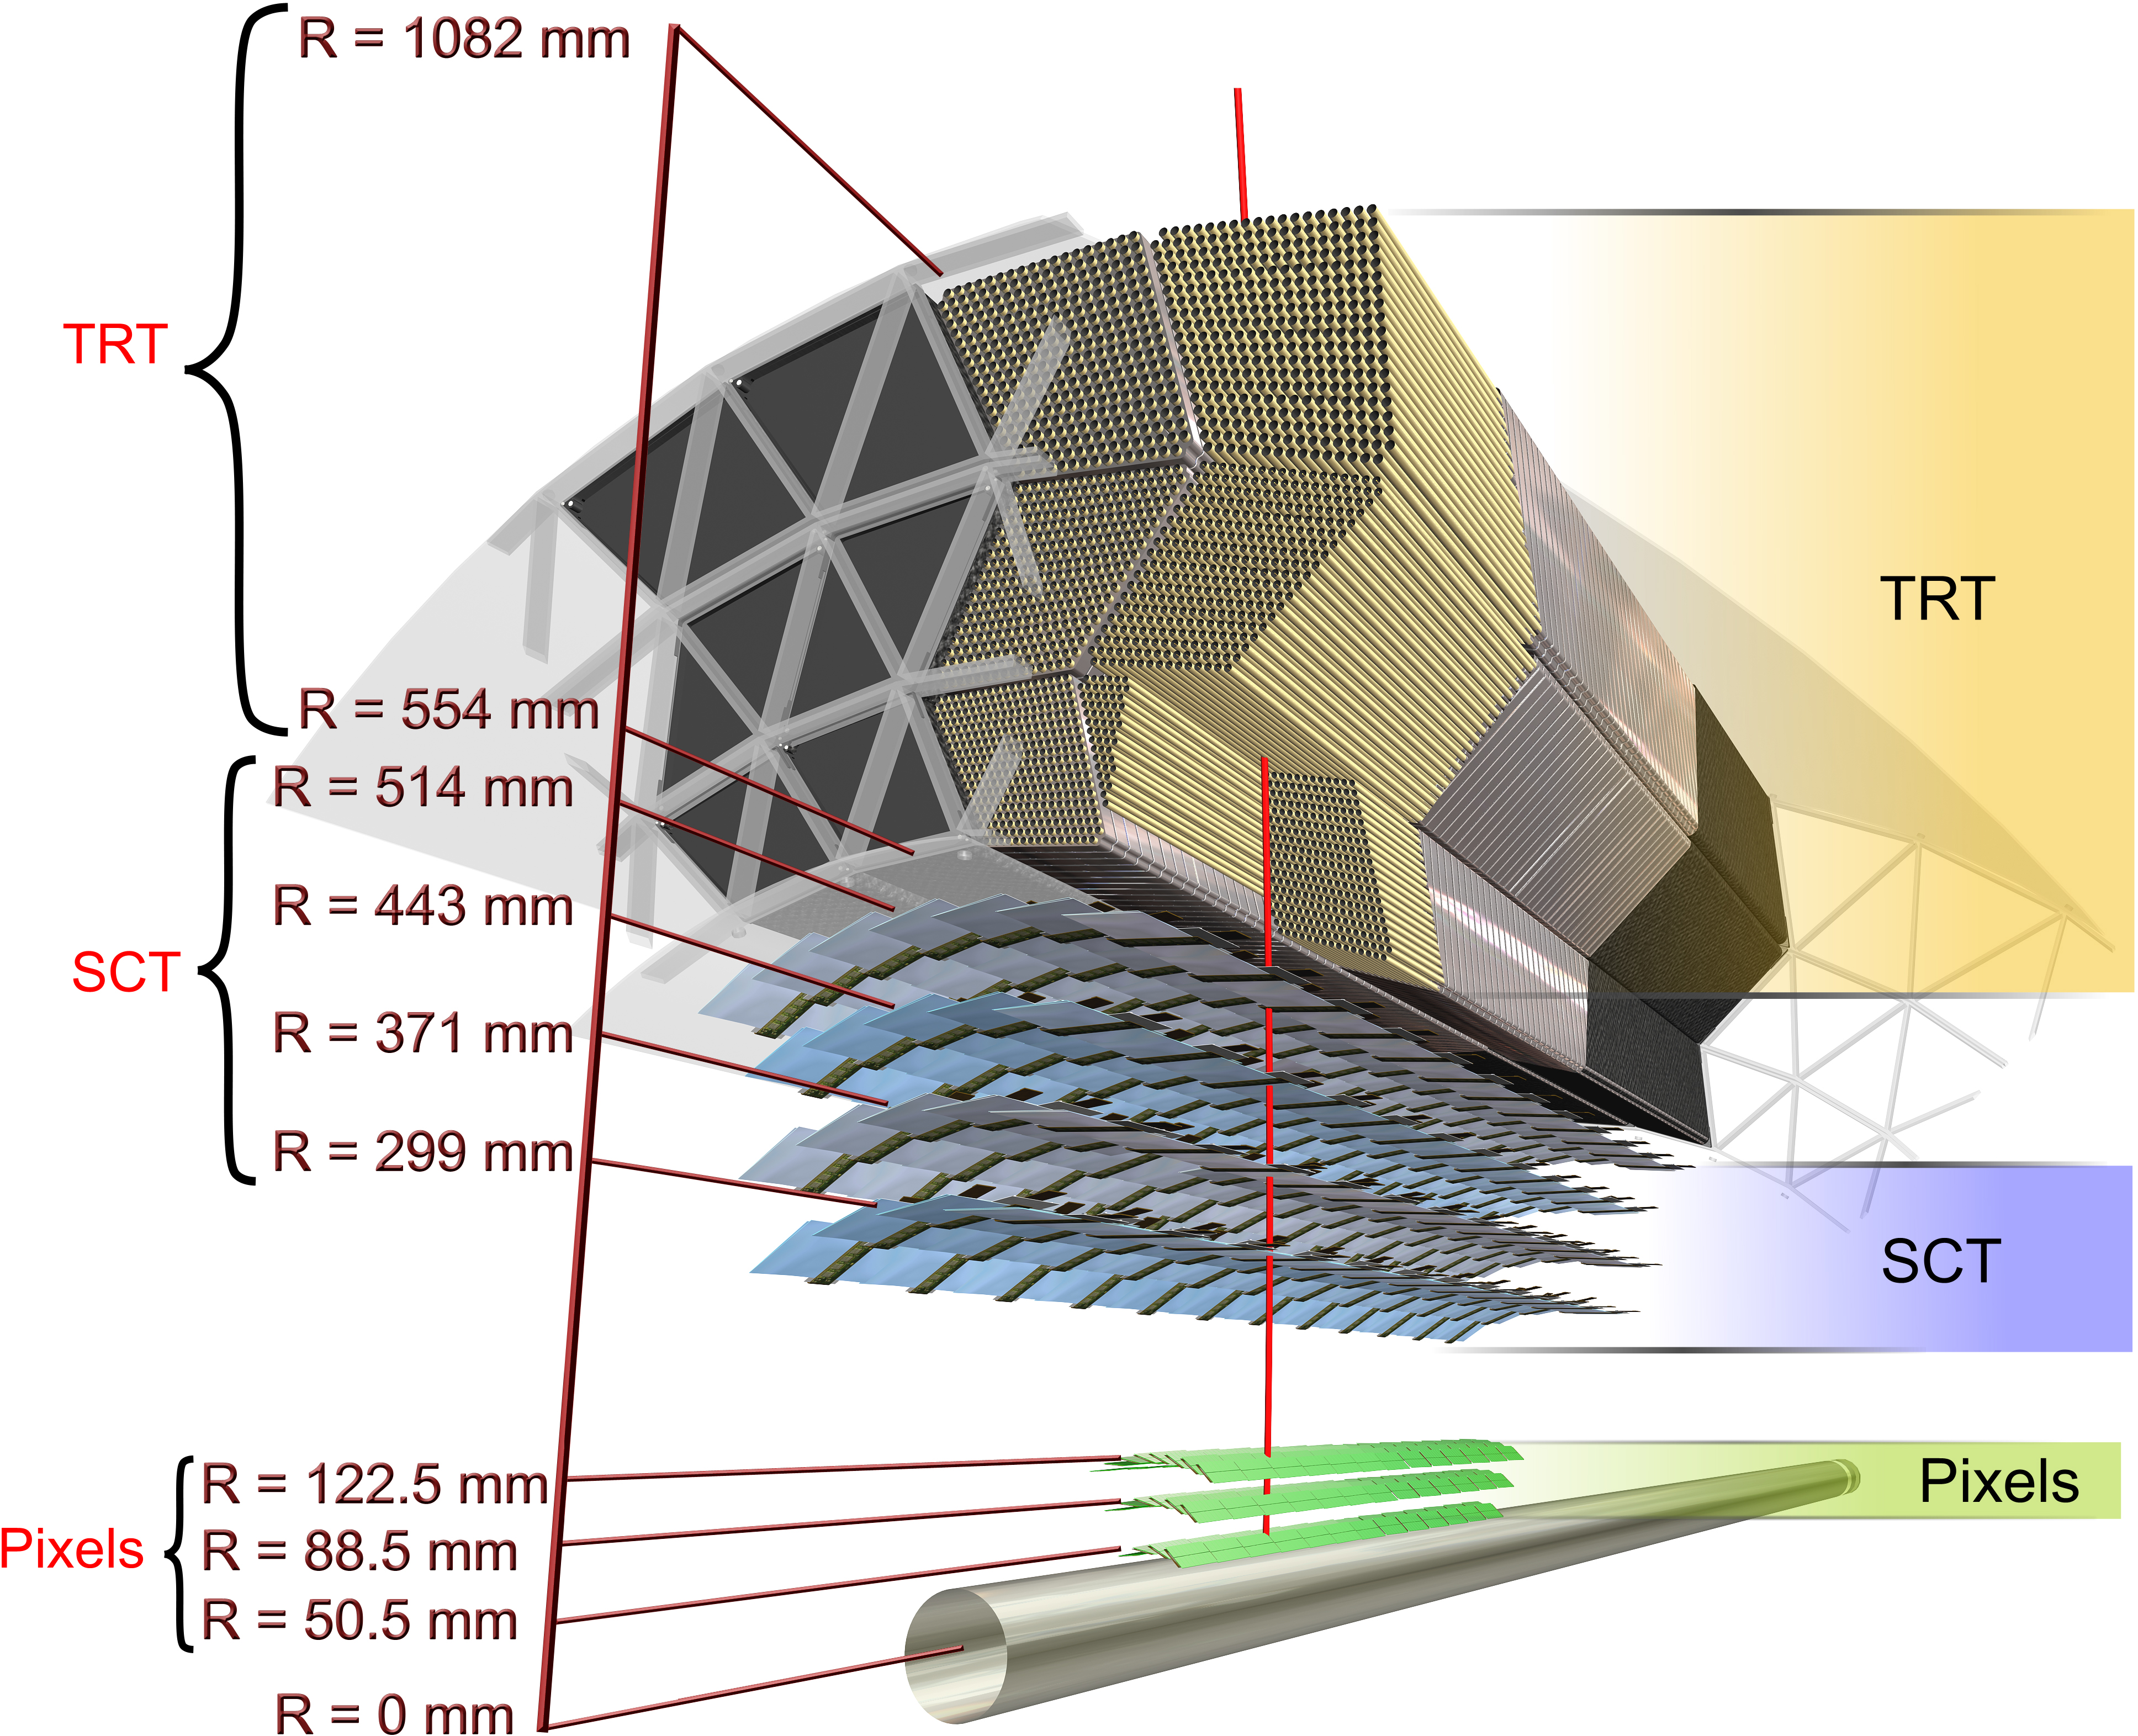
\includegraphics[width=0.84\textwidth]{figs/detector/ID.png}}
  \end{center}
  \caption[Illustration showing the ID systems being traversed by a charged track (red) of \pt=10\GeV in the barrel ($\eta$ = 0.3).]
          {Illustration showing the ID systems being traversed by a charged track (red) of \pt=10\GeV in the barrel ($\eta$ = 0.3).
          The track traverses successively the beam-pipe, the four cylindrical silicon-pixel layers (IBL included), the four cylindrical double layers of the barrel SCT, and approximately 36 axial straws contained in the barrel TRT modules within their support structure \cite{PERF-2015-08}.}
  \label{fig:detector:innerdetector}
\end{figure}

\subsubsection{Pixel Detector} \label{sec:pixel}
The closest sub-detector system to the beam line, the Pixel Detector requires the finest sensor granularity of any sub-detector on \atlas.  
Covering the $\eta$ range of $|\eta|<$2.5, the Pixel Detector is composed of four cylindrical barrel layers with 1736 sensor modules and three disk-shaped endcap layers with 288 modules.
While the detector has just 1.9~$\text{m}^2$ of total active material with pixel sizes just 50$\times$400$~\mu\text{m}^2$ for the external layers and 50$\times$250$~\mu\text{m}^2$ for the innermost layer (IBL), The Pixel Detector totals an impressive 92 million pixels (92 million electronic channels) \cite{PERF-2007-01}. 
The pixel sensors provide a resolution of 10~$\mu$m in the transverse plane, and 115~$\mu$m in the z direction (r direction) of the barrel (endcap) modules.
An illustration in Figure \ref{fig:detector:innerdetector} shows the barrel Pixel layers that reach just beyond 12 cm radially out from the beam line.

\subsubsection{Semiconductor Tracker} \label{sec:sct}
The next detector is the Semiconductor Tracker, which uses the same basic technology as the Pixels, but the fundamental unit of silicon is a ``strip.''
Covering $|\eta|<$2.5 the SCT consists of 4,088 two-sided modules and over 6 million implanted readout strips (6 million channels).
The total instrumented area of 60 square meters of silicon is distributed over 4 cylindrical barrel layers and 18 planar endcap discs.
Readout strips every 80~$\mu$m on the silicon, allowing the positions of charged particles to be recorded to an accuracy of 17~$\mu$m per layer (in the direction transverse to the strips).
Thanks to stereo information from the strips, the resolution in the z (r) direction of the barrel (endcap) modules is 580~$\mu$m.

\subsubsection{Transition Radiation Tracker} \label{sec:trt}
The Transition Radiation Tracker is the outermost and largest-by-volume system of the ID.
At a volume of 12~$\text{m}^3$ the TRT consists of 350,000 small-radius (4 mm diameter) drift tubes called ‘straws.’ Each straw functions as a simple anode (a 0.03~mm diameter gold-plated tungsten wire at the center) and cathode (outer aluminium-coated kapton film) immersed in an 'electrolyte' (a Xe-based gas mixture).
electrons drifting towards the anode.
In the strong electric field close to the anode, avalanche multiplication leads to a signal on the anode wire.
The TRT records if the signal on the wire above a low threshold every 3.25 ns.
The maximum drift time (from ionization at the edge of the straw) is 60 ns.   Transition radiation occurs for high energy electrons going through a polymer material between the straws.
Expensive Xenon gas is used in the TRT since it has a higher absorption cross section for these transition radiation X-rays than the much cheaper Argon. 
The transition radiation results in larger ionization and a larger pulse. 
The TRT records if the signal on the wire goes above a high threshold every 25 ns.
%Barrel, each straw 144 cm long. The ends of a straw are read out separately
%endcaps, each straw 39 cm long
Precision measurement of 130 microns (particle track to wire) are possible and the TRT provides electron identification information independent from the calorimeters.
%Beyond the nominal tracking measurements that the TRT provides the detector also %functions as an electron detector through the discrimination of so called low and high threshold hits.

%This radiation is absorbed by the Xe-based gas mixture filling the straws, discriminating electrons from hadrons over a wide energy range. Due to gas leaks, some TRT modules are filled with an Ar-based gas mixture.
%It also identifies tracks from secondary vertices, permitting an efficient reconstruction of photon conversions in the ID up to a radius of about 800 mm.